\chapter{Contexte de travail}
\label{sec:context}

  Pour répondre aux enjeux du passage à l'échelle, l'équipe ALSOC du LIP6
  participe à deux projets européens successifs: TSAR~\cite{tsar2008} et
  SHARP~\cite{sharp2012}. Ces projets, pour le LIP6, ont pour but de fournir une
  architecture de processeur, TSAR, de plusieurs centaines de c\oe urs, et un
  système d'exploitation pour gérer efficacement cette nouvelle architecture.
  %%\nomenclature{SHARP}{TODO}

  Notre travail portera sur ALMOS, dont l'architecture va évoluer vers celle
  d'un multi-noyau, et plus particulièrement sur la migration de tâches entre
  différentes instances du noyau. Nous allons dans un premier temps présenter
  l'architecture matérielle TSAR. L'étude de cette dernière est essentielle pour
  bien comprendre les enjeux pour ALMOS. Ensuite nous présenterons le noyau
  d'ALMOS, et enfin nous concluerons sur le travail que nous allons effectuer
  dans le cadre de ce stage.
  

  \section{L'architecture TSAR}
  \label{sec:tsar}

    TSAR est l'architecture d’un processeur multi-c\oe urs cc-NUMA homogène
    pouvant intégrer jusqu’à 1024 c\oe urs~\cite{greiner2009tsar}. Cette
    architecture est le résultat de deux projets de recherche européens
    MEDEA+~\cite{tsar2008,sharp2012} dont les principaux partenaires industriels
    sont BULL, Philips et THALES, et dont les partenaires académiques sont le
    LIP6 et le CEA-Leti. La figure \ref{fig:tsar} est un aperçu global de
    l'architecture TSAR. Il s'agit d'un ensemble de clusters interconnectés par
    un NoC\nomenclature{NoC}{Network-On-Chip}
    DSPIN\nomenclature{DSPIN}{Distributed Scalable Predictable Integrated
      Network}. Chaque c\oe ur dispose de ses propres caches L1 indexés en
    adresses physiques (données et instructions séparées) et d'une MMU. La
    cohérence des caches de premier niveau de tous les c\oe urs ainsi que des
    TLBs\nomenclature{TLB}{Translation Lookaside Buffer} est assurée par un
    protocole matériel nommé DHCCP\nomenclature{DHCCP}{Distributed Hybrid Cache
      Coherence Protocol}. Une description complète de cette architecture est
    disponible sur le site du projet TSAR~\cite{tsar2008web}.

    \begin{figure}[ht]
      \centering 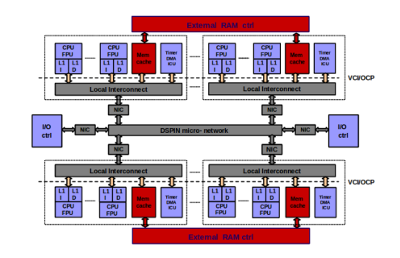
\includegraphics[scale=0.241]{include/img/tsar.png}
      \caption{Schéma global de l'architecture TSAR. Les clusters sont composés
        de quatre processeurs connectés entre eux sur un interonnect local,
        lui-même relié à différents périphériques (TTy, ICU, NIC,
        etc\ldots)~\citep{greiner2009tsar}.}
      \label{fig:tsar}
    \end{figure}
    \nomenclature{TTy}{TeleTYpe} \nomenclature{ICU}{Interrupt Control Unit}
    \nomenclature{NIC}{Network Interface Controller}

    Dans la suite de ce document, on considére la version TSAR-Leti comme étant
    l'architecture de référence. Celle-ci contient jusqu'à 1024 c\oe urs MIPS32
    répartis en 256 clusters de 4 c\oe urs chacun. La mémoire physique
    adressable est de 1To, et chaque cluster gère un segment de 4Go


  \section{Le noyau ALMOS}
  \label{sec:almos}

    Le noyau ALMOS~\cite{almaless2011almos,almaless2014universite} est un noyau
    monolithique expérimental developpé au LIP6 dans l'équipe ALSOC depuis 2011
    dans le cadre de la thèse de Ghassan~\citeauthor{almaless2014universite}. Le
    développement est maintenant à la charge de Mohamed Karaoui (système de
    fichiers) et Clément Devigne (exécution de machines virtuelles). Le but
    d'ALMOS est de répondre au problème de la localité des accès mémoires dans
    les machines cc-NUMA. Une des particularités dans les choix architecturaux
    d'ALMOS est d'avoir développé un noyau monolithique. Il respecte la norme
    POSIX~\cite{posix2013} et implémente différentes libraires:
    \texttt{libpthread, mpi, openMP}\ldots Le but premier d'ALMOS est de
    garantir un passage à l'échelle et une conservation de la localité des accès
    mémoires. Pour cela, le noyau intègre trois nouveaux mécanismes:
    \benumline \item les clusters managers \item les réplica-noyau \item une
    nouvelle stratégie d'allocation mémoire (\textit{Auto-Next-Touch})
    \eenumline.

    
    \subsection{Les cluster-manager}

      L'organisation distribuée du noyau ALMOS s’appuie sur les objets nommés
      \textit{cluster-manager}. L’objectif est d’une part, de décentraliser la
      gestion des ressources et d’autre part, d’assurer une localité d’accès
      mémoire lors de cette gestion. Un cluster-manager est un objet responsable
      de la gestion des ressources physiques (essentiellement c\oe urs et
      mémoire physique) d’un n\oe ud cc-NUMA. Il existe autant de cluster-manager
      qu’il y a de clusters. Chacun d'eux est placé localement dans la mémoire
      physique de son n\oe ud. Comme l'illustre la
      figure~\ref{fig:cluster_manager}, ils contiennent, entre autre, un
      \textit{memory-manager} et un ou plusieurs \textit{core-manager}.  Le
      \textit{memory manager} est responsable de l'allocation et la gestion de
      la mémoire sur le cluster. Le \textit{core-manager} est responsable de la
      gestion d’un c\oe ur, et plus précisément de l'ordonnancement des tâches
      qui lui sont affectées. Il assure également la gestion des événements. %%Au
      %% sein de cet object, l'ordonnancement est assuré par un serveur
      %% d'ordonnancement appelé \textit{scheduler-server}, tandis que la
      %% gestion des événements est assurée par \textit{l'events-manager}.

      \begin{figure}[ht]
        \centering
        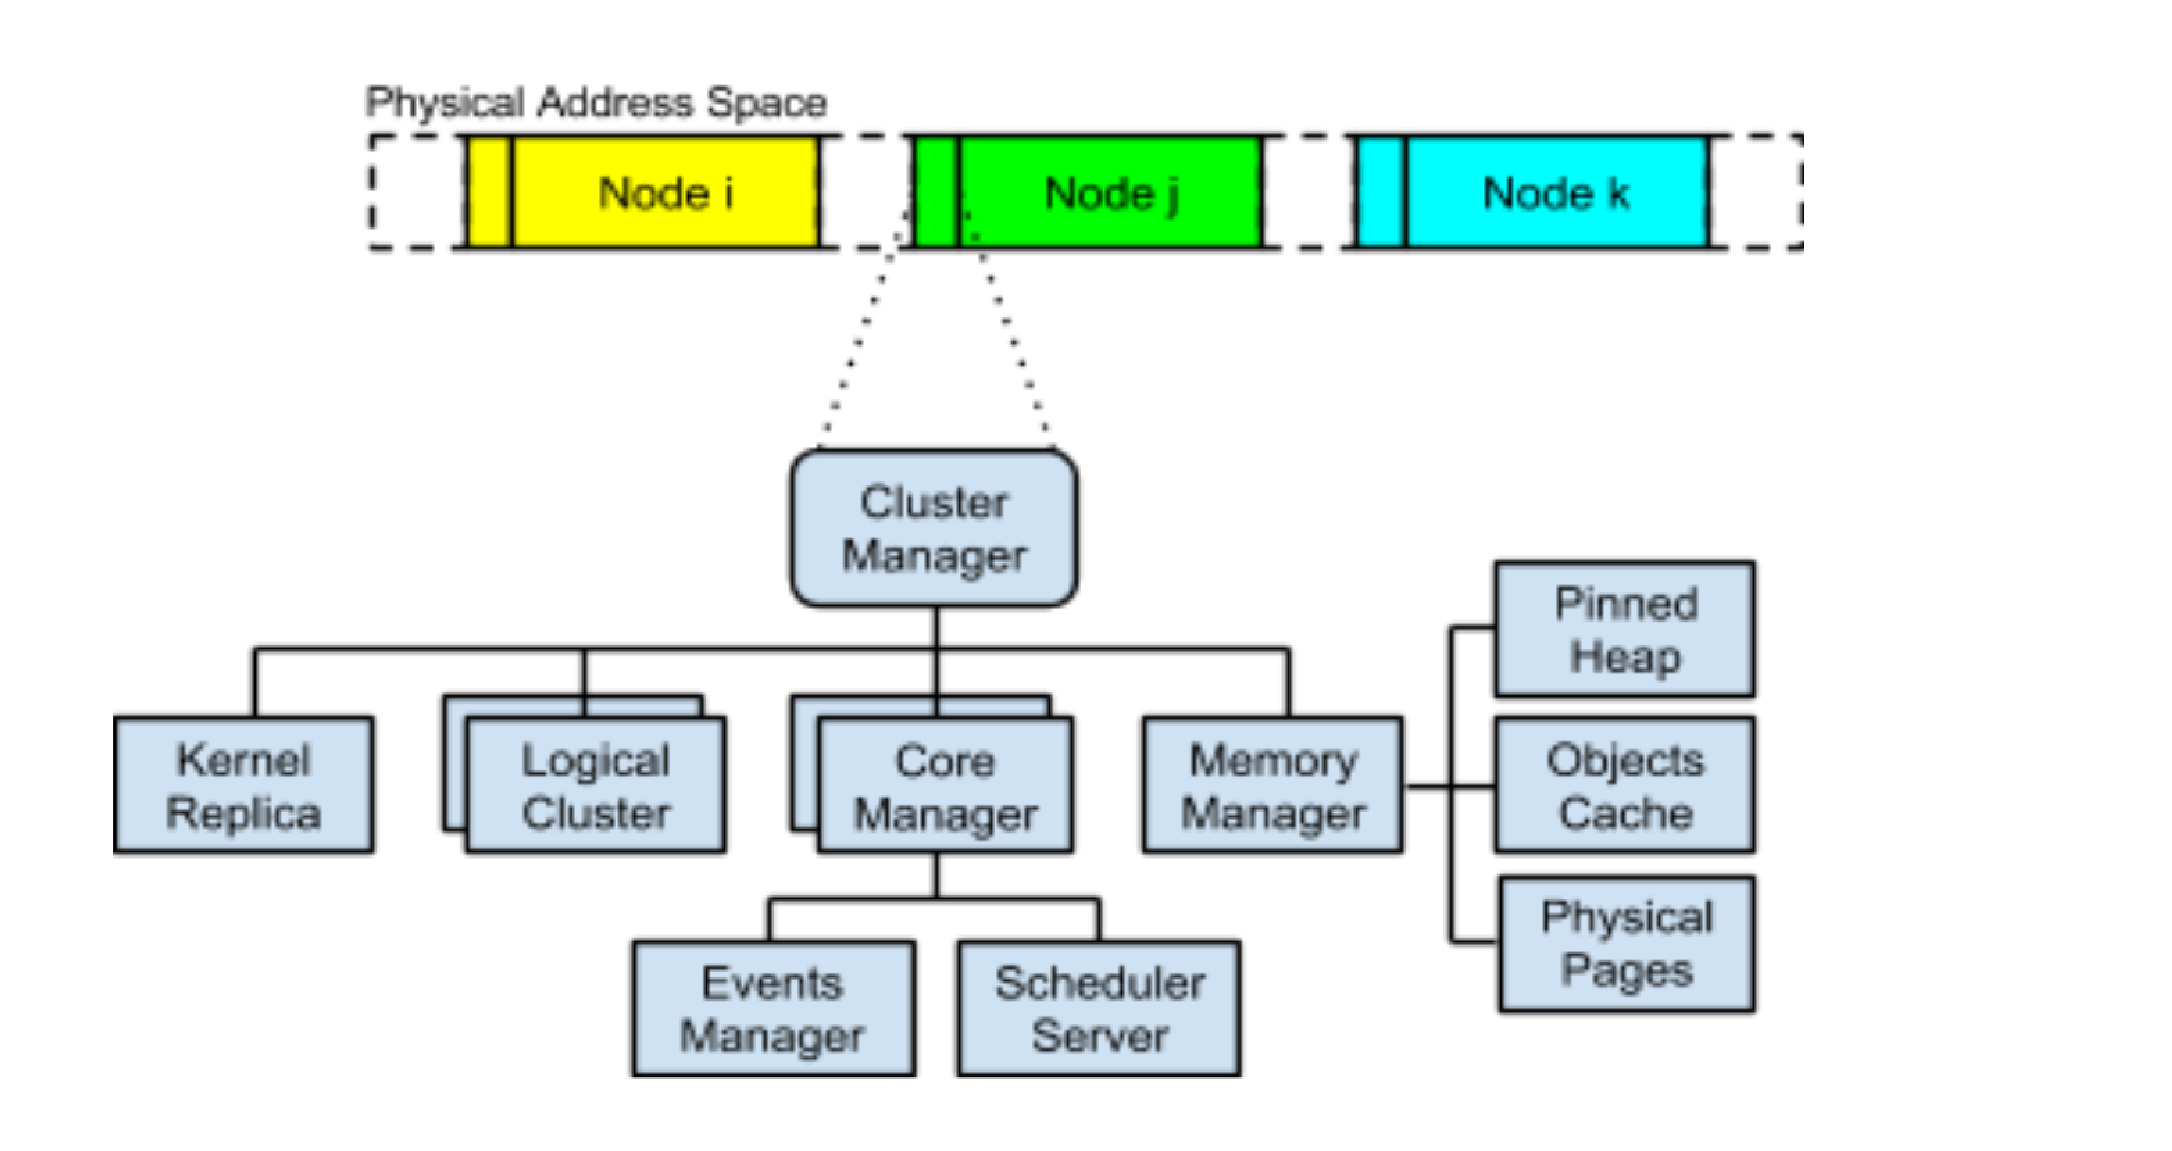
\includegraphics[scale=0.8]{include/img/cluster_manager}
        \caption{Un \textit{cluster manager} est un gestionnaire de ressources
          d'un n\oe ud cc-NUMA. Il est physiquement placé dans le banc mémoire
          du n\oe ud correspondant~\citep{almaless2014universite}.}
        \label{fig:cluster_manager}
      \end{figure}

      
    \subsection{Les réplicas noyau}

      Comme nous l'avons vu précédemment, l'architecture TSAR est clusterisée.
      Dans l'espace d'adressage d'un processus, il y a un mapping sur les pages
      du noyau, de sorte que si le code et les données du noyau sont situés à un
      seul et unique endroit en mémoire physique, et que chaque processus mappe
      ces pages dans son espace virtuel, alors on paye le coût de l'architecture
      NUMA à chaque appel système, puisque l'on doit accéder à des pages
      distantes.

      Afin de résoudre ce problème, la notion de réplica noyau a été introduite
      au sein des \textit{clusters-manager}. Un réplica noyau consiste à
      dupliquer le code du noyau et les données partagées dans les premières
      pages physiques de chaque cluster. Ces pages sont en lecture seule pour
      garantir la cohérence et la sécurité. Lors de la création d'un processus,
      les pages qui représentent le noyau correspondent aux pages physiques du
      cluster sur lequel le processus vient d'être créé.


  \section{Évolution du projet}

    \subsection{Limitations de la version initiale}
    
      Développé initialement sur une architecture avec 4Go de mémoire physique,
      le noyau ne peut pas supporter plus de 4Go de mémoire vive. L'objectif
      visé n'était pas de supporter le tera-octet de mémoire de TSAR, mais de
      supporter le passage à l'échelle de plusieurs centaines de c\oe
      urs. Ainsi, un des premiers problèmes d'ALMOS est le mapping de l'espace
      virtuel. En effet, lors de la phase de boot, ce dernier cherche à mapper
      toute la mémoire physique du cluster de boot dans son espace
      virtuel. Contraitement aux noyaux ``classiques'', ALMOS s'accorde 2Go
      d'espace virtuel au lieu de 1. Donc, si ce cluster possède (au moins) 2Go
      de mémoire physique, l'ensemble du noyau est mappé dans ce seul
      cluster. Enfin, cela ne laisse que 2Go de mémoire virtuelle pour les
      applications utilisateur.

      
    \subsection{Contributions de François~\citeauthor{guerret2014exploitation}}
      
      La gestion d'une mémoire physique de 1To a été le sujet de stage de
      François~\citet{guerret2014exploitation} en 2014. Ce dernier a proposé
      différents changements pour ALMOS (figure~\ref{fig:almos-guerret}):
      \benumline \item réduire l'espace virtuel du noyau à 1Go \item répartir
      cet espace virtuel entre les clusters \item sortir de l'espace virtuel les
      structures de données du noyau de taille importante \eenumline.

      \begin{paragraph}{Répartition de l'espace d'adressage noyau:}
        Elle est calculée en fonction du nombre de clusters de l'architecture
        ($\frac{\text{Taille virtuelle}}{\text{Nb clusters}}$). Pour une
        architecture TSAR-Leti 40 bits, on dispose de 256 clusters, on a donc
        $\frac{1000}{256}\approx4$Mo d'espace virtuel pour le noyau par cluster.
      \end{paragraph}

      \begin{figure}[ht]
        \centering 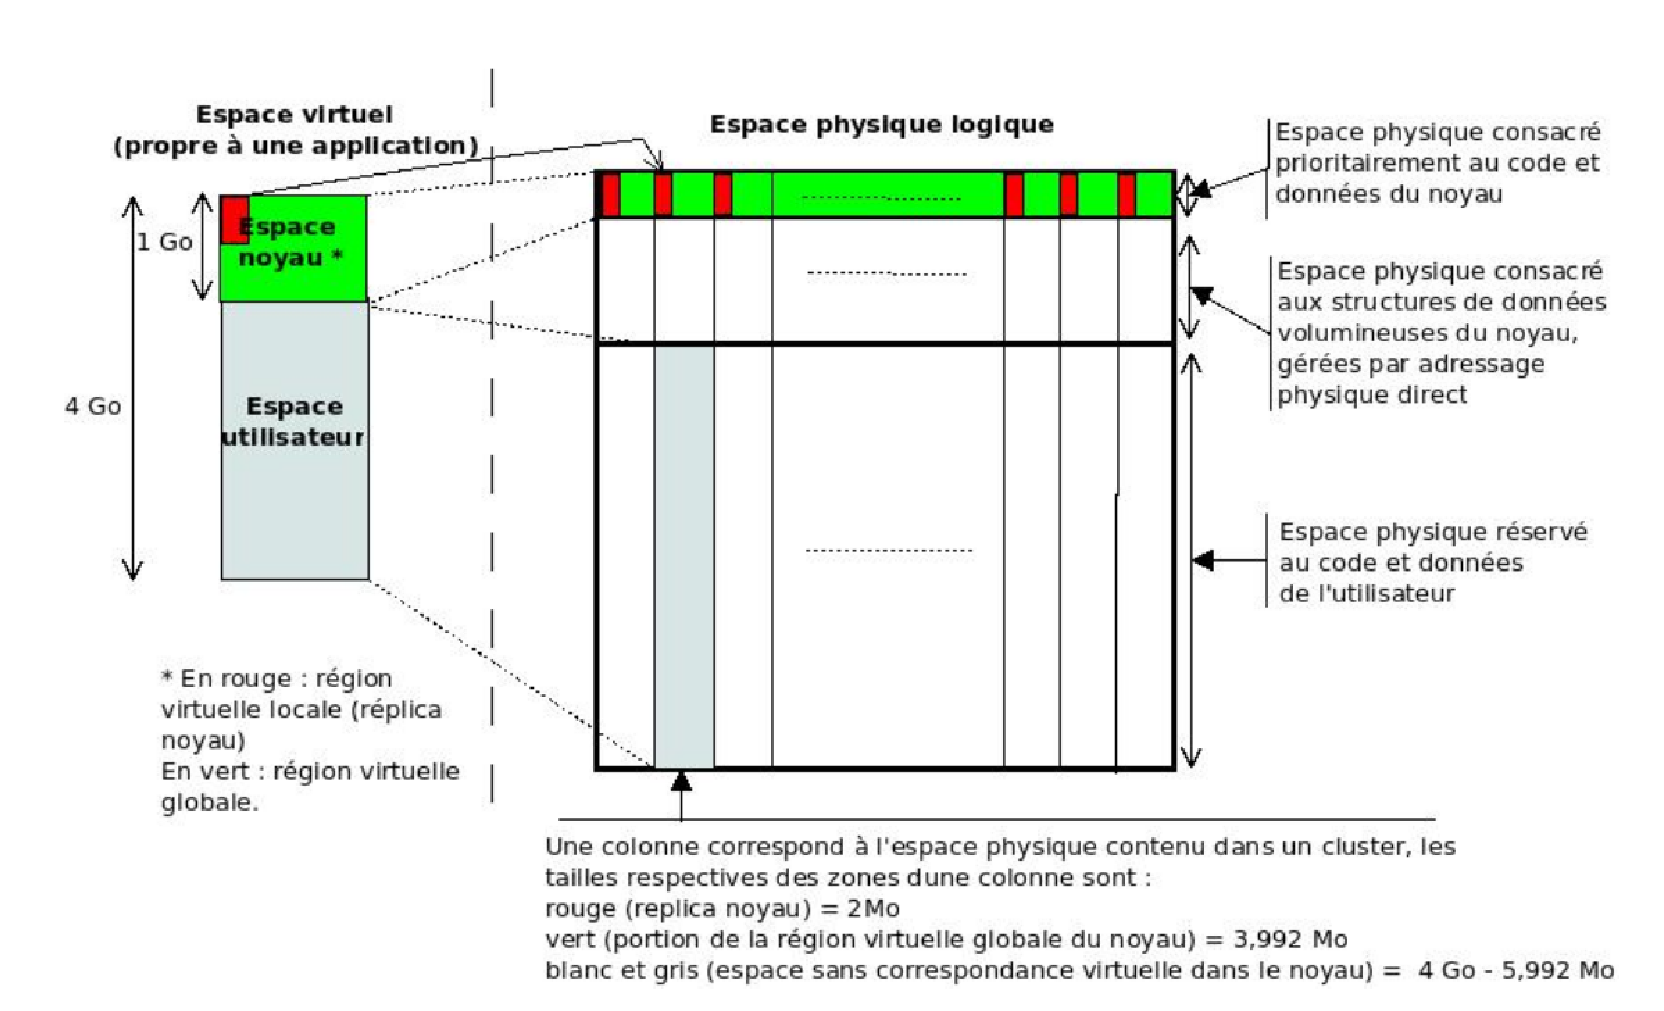
\includegraphics[scale=0.8]{include/img/almos-guerret}
        \caption{Répartition de l'espace virtuel du noyau tel que proposé par
          François \citet{guerret2014exploitation}.}
        \label{fig:almos-guerret}
      \end{figure}

      \begin{paragraph}{Gestion en adressage physiques de structures de données:}
        Avec seulement 4Mo d'espace virtuel pour le noyau par clusters,
        certaines structures de données ne pouvent plus être contenues dans un
        si petit espace, comme par exemple la table des pages d'un
        processus. Celle-ci, une fois pleine\footnote{Ce cas n'arrive jamais,
          mais il est néanmoins théoriquement possible}, peut atteindre jusqu'à
        8Mo. De plus, chaque processus dispose de sa propre table des pages. Il
        est techniquement impossible de stocker 8Mo dans 4Mo, François a donc
        choisi de sortir cette structure de l'espace virtuel.

        La seconde structure de données problématique est la table des
        descripteurs de pages physiques. Les noyaux monolithiques, dont ALMOS,
        ont fait le choix de décrire dans une structure à plat toutes les pages
        physiques qu'offre la mémoire. Ainsi, pour décrire le tera-octet de
        mémoire offert par TSAR, il est nécessaire d'utiliser 14Go de mémoire,
        soit 56Mo par cluster. Une fois de plus, il est impossible de stocker
        cette structure dans l'espace virtuel noyau. Celle-ci en a donc été
        sortie et est gérée en adressage physique.
      \end{paragraph}

      \begin{paragraph}{Résultats:}
        Ce travail n'a malheureusement pas donné lieu à une solution
        fonctionnelle. La gestion par des adresses physiques de ces deux
        structures s'est avérée être très compliquée et nécessitait de recoder
        une partie conséquente du noyau. Le principal inconvénient est le
        parcours de listes: il est nécessaire de vérifier que chaque élément
        n'est pas une structure gérée physiquement avant de pouvoir y
        accéder. Cela allourdi considérablement l'opération, cette solution a
        donc été donc abandonnée. Néanmoins, elle a posée les bases de la
        version suivante d'ALMOS.
      \end{paragraph}

      
  \section{Passage au mode multi-noyau}
  \label{sec:multi-noyau}

    La version actuelle d'ALMOS proposée par Mohamed Karaoui supprime totalement
    l'espace virtuel pour le noyau. Ce dernier fonctionne entièrement en
    adressage physique et de ce fait passe en mode multi-noyau, avec une
    instance de noyau par cluster. Ces changements permettent de gérer toute la
    mémoire physique de la plateforme TSAR, puisque: \benumline \item chaque
    cluster dispose de 4Go de mémoire physique \item on a un noyau par
    cluster \item le noyau peut gérer 4Go de mémoire\eenumline. Ces changements
    permettent également de laisser 4Go de mémoire virtuelle\footnote{Modulo une
      page de petite taille (4Ko) pour faire le passage entre le mode
      utilisateur et le mode noyau} à l'utilisateur puisque le noyau ne
    l'utilise plus.\\

    En revanche, cette solution soulève une difficulté majeure. En choisissant
    de clusteriser le noyau, on rend impossible la communication directe par
    simples load-store à la mémoire des clusters voisins. En effet, avec un
    noyau par cluster, les espaces d'adressage deviennent propres à ces
    derniers, et la vision simple d'un espace d'adressage unique entre les
    clusters n'existe plus. On ne peut donc plus accéder aux éléments des autres
    clusters de manière directe et transparente. Il existe alors deux méthodes
    complémentaires:\benumline \item utiliser une propriété du cache L1 de TSAR
    permettant de former une adresse physique quelconque ou \item utiliser le
    passage de messages entre les instances du noyau\eenumline.\\

    Une seconde conséquence de ce choix est d'avoir rendu non fonctionnelle la
    migration de processus et de threads entre les clusters (la migration entre
    c\oe urs d'un même cluster est toujours fonctionnelle). Dans la version
    initiale d'ALMOS, cette migration se faisait:\benumline \item en stoppant le
    processus sur le c\oe ur concerné puis \item en l'ajoutant dans la liste des
    processus du c\oe ur distant et \item en relancant son exécution sur ce
    nouveau c\oe ur\eenumline. L'ajout du processus dans cette liste est
    possible uniquement parce que le noyau est en mémoire virtuelle. Il peut
    ainsi accéder au \textit{core-manager} du cluster destinataire sans se
    rendre compte que celui-ci est distant, et lui ajouter la \texttt{struct
      task} du processus à migrer. Les pages physiques du processus seront
    ensuite migrées via la stratégie \textit{Auto-Next-Touch}.\\

    En choisissant de passer ALMOS en mode multi-noyau, chaque cluster est géré
    par un noyau différent. Les clusters ont par conséquent des espaces
    d'adressage différents, ce qui modifie les mécanismes de migration de
    processus ou de threads. C'est à cette problématique que nous allons
    répondre.


  \section{Objectifs}

    La problématique soulevée en~\ref{sec:multi-noyau} est celle à laquelle nous
    allons répondre dans le cadre de ce stage. Plus précisément, il s'agit de
    définir et de mettre en place les mécanismes suivants:

    \begin{itemize}
      \item assurer la création et la migration de processus mono-threads entre
        clusters
      \item ajouter le support du multi-threading
      \item ré-implémenter le composant d'ALMOS appelé
        DQDT\nomenclature{DQDT}{Distributed Quaternary Decision Tree}, assurant
        la vision globale de l'occupation des ressources matérielles de la
        plateforme, et par conséquent reponsable du placement des ressources sur
        celle-ci.
    \end{itemize}

    %% Pour plus de détails sur la spécification du problème ainsi que son
    %% implémentation, on peut se référer à~\citep{peneau2015todo}.
